% 1000 words
To recapitulate our findings thus far: First, we have established that provided with open data on population, amenity points-of-interest density and diversity, and select public transportation accessibility indices, we can predict the total number of arrivals by public transport to a high degree of accuracy using an XGBoost model that is fine-tuned to overcome overfitting due to highly correlated features. The transformation of the target variable and the inclusion of spatial lag features were essential to achieving a high $R^2$ greater than 0.8 even after already accounting for spatial autocorrelation using nested k-fold cross-validation to avoid inflated performance metrics. Secondly, using SHAP for machine learning model explanation, we managed to extract more sophisticated feature importance indications than originally available with XGBoost. Furthermore, by examining local SHAP explanations, we can identify hotspots for different POI features overall and across different time bands. 

One of the benefits of using SHAP values as imperfect approximants to coefficients in a statistical model is their additive nature. This means that we can decompose the model's predictions into the sum of the SHAP values, with which we can control for unwanted effects. For example, without an explicit origin-destination matrix and dwell time data and using only station exits and bus alighting data, it is not immediately possible to say whether a person is exiting at a destination to attend an activity or to interchange to another mode of transport. Using SHAP to extract local importance with its additive property can help consider the impact of the amenity profile of the destination area on the trip attractiveness of the area while controlling for the connectivity profile of the area. 

\begin{figure}[!ht]
    \centering
    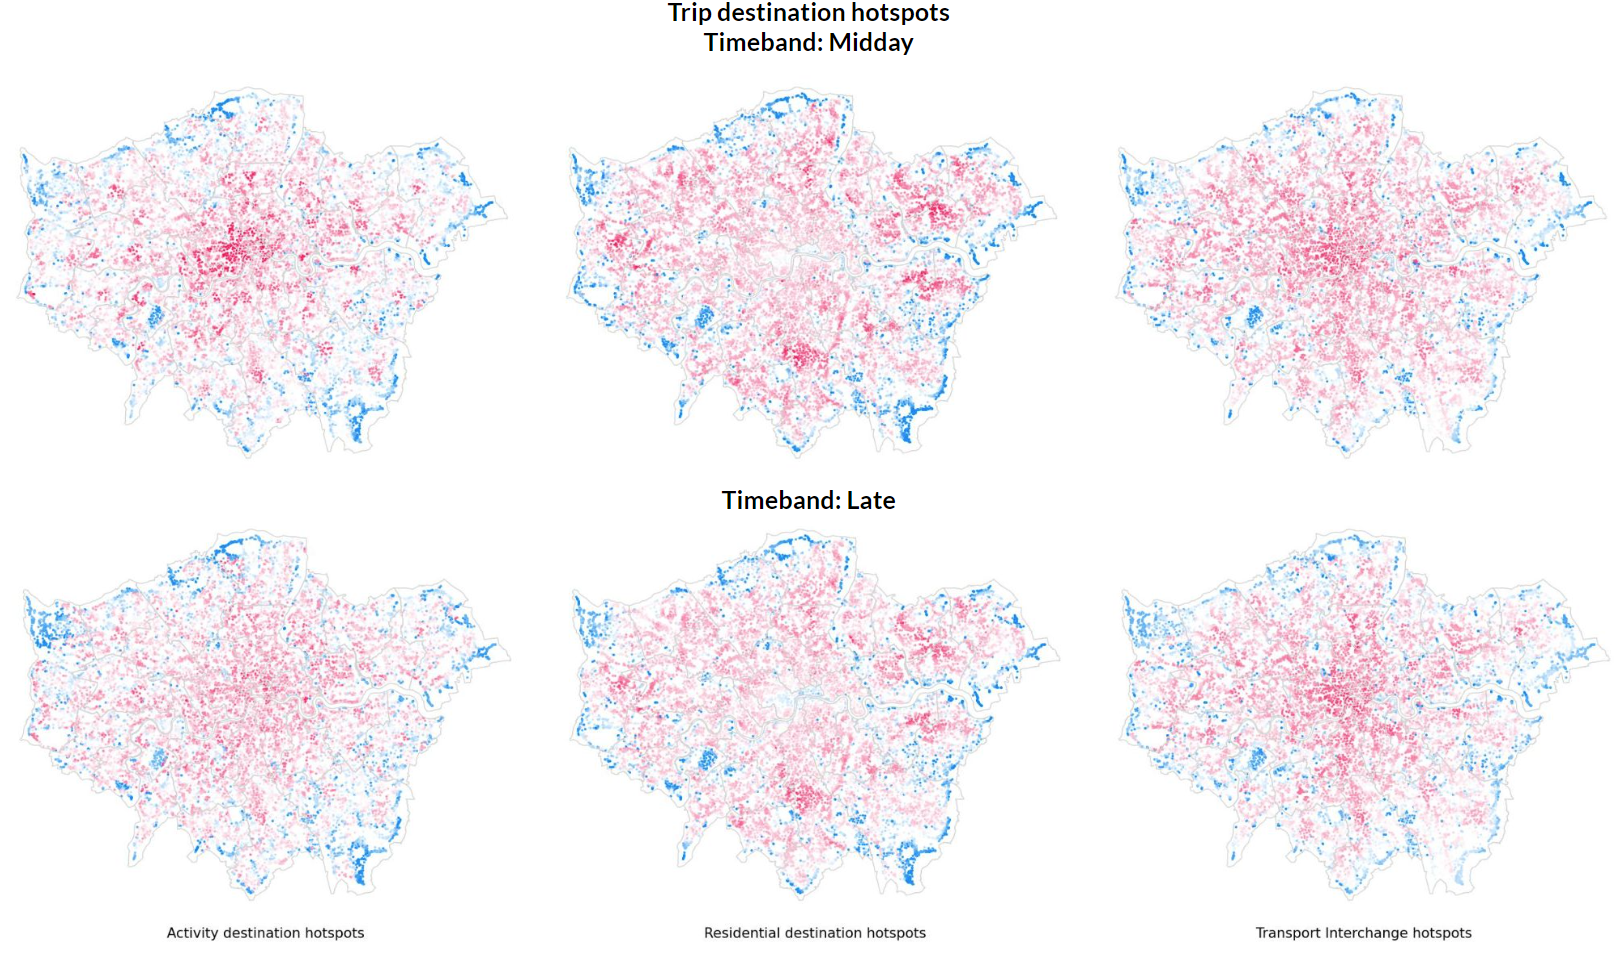
\includegraphics[width=0.75\textwidth]{destinationhotspot.png}
    \captionsetup{justification=centering}
    \caption{Hot spots for destination groups: Amenity vs. Residential vs. Transport\\ Midday vs Late}
    \label{fig:destinationhotspot}
\end{figure}

One way to visualise it is by grouping local SHAP values by feature groups and visualising their spatial distribution. This can be seen in Figure \ref{fig:destinationhotspot} with features grouped into (1) amenity-related, (2) population-related, and (3) connectivity-related features. When comparing Midday and Late time bands, we can see that the trip attractiveness of areas because of their connectivity profile is relatively unchanged, whereas the trip attractiveness of areas because of their amenity profile is significantly more pronounced in the Midday time band, despite the fact that connectivity-related features have high global importance. This suggests that we can segment whether an area attracts public arrivals because of their amenities or their connectivity in the network. This is useful for instances where we want to qualify certain popular areas as destination hotspots based on the availability of amenities alone. 

Applying spatial clustering such as HDBSCAN of spatial units based on their amenity-related compound SHAP values can effectively surface activity hotspots in a given area in Greater London that are destinations for (non-commute) public transport trips. Figure \ref{fig:woodgreen} demonstrates the activity hotspot in Wood Green with the highest mean amenity-related SHAP values, made up of 5 constituent spatial units (isochrones). This can be useful for local authorities to identify areas that are popular with public transport users for non-commute activities, such as shopping, dining, or entertainment.

\begin{figure}[!ht]
    \centering
    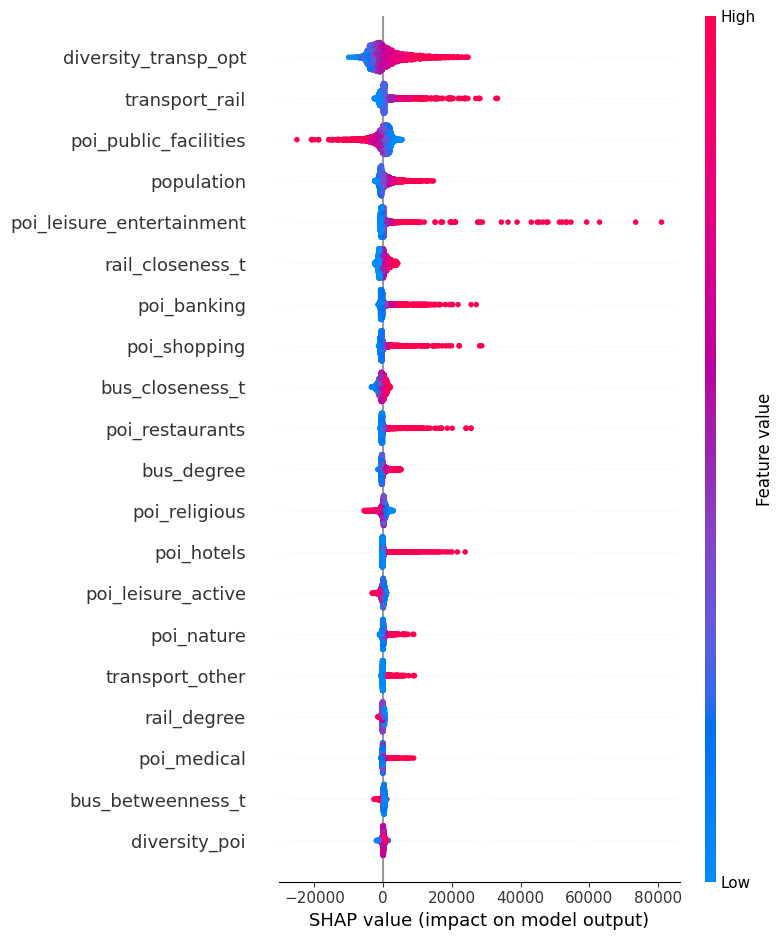
\includegraphics[width=0.8\textwidth]{output.png}
    \captionsetup{justification=centering}
    \caption{Identifying high activity areas in Wood Green}
    \label{fig:woodgreen}
\end{figure}

Finally, it is worth acknowledging the limitations of the methodology that affect its generalisability and applicability in certain cases, many of which have been discussed in the previous sections.

\begin{itemize}
    \setlength\itemsep{0em}
    \item \textit{Missing features}: The analysis of outliers suggests that there are other factors that may be influencing the number of arrivals in an area that are not accounted for in the model. These could include socioeconomic factors, car ownership, or other urban morphological features that affect people's usage of public transport.
    \item \textit{Generalisability}: The high feature importance of the spatial lag features across the board means that the model may not be able to accurately predict a new observation in isolation from its neighbours, nor can it be readily generalisable to other cities. Nevertheless, the model can be used to predict the trip attractiveness of a given area in Greater London as the city changes, giving transport planners a useful tool. For example, when a neighbourhood is undergoing redevelopment, we can predict the potential inflow of public transport trips based on the planned addition of amenities or transport facilities.
    \item \textit{Causality}: However, the lack of consideration for causality means that we cannot infer that the presence of a certain amenity of a certain density will cause more arrivals to a certain area. Rather, we can only observe which amenity or connectivity features among those included in the training of the model are the best predictors of arrivals in an area.
    \item \textit{POI classification}: The classification of amenity and transport POIs in this analysis adheres to Geofabrik's OSM data classification. Future work could attempt to reclassify these POIs in a deliberate manner to capture the association between certain trip purposes of interest and the types of urban amenities that fulfil them.
    \item \textit{Types of mobility}: Our analysis uses public transport demand data from one agency (TfL) over a typical Saturday to approximate non-commute public transport trips, meant to remove the effect of employment centres from the analysis as much as possible. However, this does not account for other types of mobility, such as cycling, walking, or driving, which may be more prevalent on weekends, nor does it account for those who work on weekends. Future work could incorporate mode-agnostic mobility data together with trip purpose inferences to exact more precise non-commute trip attractiveness predictions.
\end{itemize}